% !TeX program = xelatex
% !BIB program = biber
% !TeX encoding = UTF-8

% =============================================================================
% Template LaTeX IPG  —  https://github.com/VagnerBomJesus/TEMPLATE-IPG-LATEX
% Autor base, criador e mantenedor do projeto:
%     Vagner Bom Jesus  (@VagnerBomJesus)
%
% Proprietario e autor original deste template. Ao reutilizar, distribuir ou
% editar, MANTER este credito ao autor base (nao remover). Quem usa o template
% e o autor do SEU relatorio; o criador base do modelo e Vagner Bom Jesus.
% Licenca: GPL-3.0 (ver LICENSE).
% =============================================================================

% =============================================================================
% Template LaTeX — Mestrado em Computação Móvel
% Instituto Politécnico da Guarda (IPG)
% Escola Superior de Tecnologia e Gestão (ESTG)
% =============================================================================

\documentclass[12pt,a4paper,twoside,openright]{book}

% --- Dados do documento (preencher aqui) ---
\newcommand{\tituloRelatorio}{Título do Relatório}
\newcommand{\subtituloRelatorio}{Subtítulo se necessário} % deixar vazio {} se não houver subtítulo
\newcommand{\nomeAutor}{Nome Completo do Autor}
\newcommand{\numeroAluno}{Número do Aluno}
\newcommand{\nomeOrientador}{Prof. Doutor Nome Completo}
\newcommand{\nomeCoorientador}{Prof. Doutor Nome Completo} % remover da capa se não houver coorientador
\newcommand{\mesAno}{Junho | 2025}
\newcommand{\anoLetivo}{2024/2025}
\newcommand{\tipoRelatorio}{Relatório de Projeto Aplicado} % opções: Relatório de Projeto Aplicado | Estágio Profissionalizante | Dissertação

% --- Carregar preâmbulo (pacotes e configurações) ---
% =============================================================================
% Template LaTeX IPG  —  https://github.com/VagnerBomJesus/TEMPLATE-IPG-LATEX
% Autor base, criador e mantenedor do projeto:
%     Vagner Bom Jesus  (@VagnerBomJesus)
%
% Proprietario e autor original deste template. Ao reutilizar, distribuir ou
% editar, MANTER este credito ao autor base (nao remover). Quem usa o template
% e o autor do SEU relatorio; o criador base do modelo e Vagner Bom Jesus.
% Licenca: GPL-3.0 (ver LICENSE).
% =============================================================================

% =============================================================================
% Preâmbulo — Pacotes e Configurações
% IMPORTANTE: requer XeLaTeX ou LuaLaTeX (NÃO pdflatex)
% =============================================================================

% --- Língua ---
\usepackage[portuguese]{babel}

% --- Fontes (requer XeLaTeX/LuaLaTeX + fontspec) ---
\usepackage{fontspec}
\setmainfont{Times New Roman}
\setsansfont{Calibri}[
    BoldFont       = Calibri Bold,
    ItalicFont     = Calibri Italic,
    BoldItalicFont = Calibri Bold Italic
]
\setmonofont{Courier New}

% --- Geometria da página ---
\usepackage[a4paper,top=2.5cm,bottom=2.5cm,inner=3cm,outer=2.5cm]{geometry}

% --- Espaçamento entre linhas ---
\usepackage{setspace}
\onehalfspacing

% --- Headings (titlesec) ---
\usepackage{titlesec}
\titleformat{\chapter}[block]{\sffamily\bfseries\fontsize{18}{22}\selectfont}{\thechapter.}{0.5em}{}
\titlespacing*{\chapter}{0pt}{0pt}{18pt}
\titleformat{\section}{\sffamily\bfseries\fontsize{16}{20}\selectfont}{\thesection}{0.5em}{}
\titlespacing*{\section}{0pt}{18pt}{6pt}
\titleformat{\subsection}{\sffamily\bfseries\fontsize{14}{18}\selectfont}{\thesubsection}{0.5em}{}
\titlespacing*{\subsection}{0pt}{14pt}{4pt}
\titleformat{\subsubsection}{\sffamily\fontsize{12}{15}\selectfont}{\thesubsubsection}{0.5em}{}
\titlespacing*{\subsubsection}{0pt}{12pt}{4pt}
\titleformat{\paragraph}[hang]{\sffamily\fontsize{12}{15}\selectfont}{\theparagraph}{0.5em}{}
\titlespacing*{\paragraph}{0pt}{10pt}{4pt}

% --- Cabeçalhos e rodapés — Calibri 10pt ---
\usepackage{fancyhdr}
\pagestyle{fancy}
\fancyhf{}
\fancyhead[LE]{\sffamily\fontsize{10}{12}\selectfont\leftmark}
\fancyhead[RO]{\sffamily\fontsize{10}{12}\selectfont\rightmark}
\fancyfoot[C]{\sffamily\fontsize{10}{12}\selectfont\thepage}
\renewcommand{\headrulewidth}{0.4pt}
\renewcommand{\footrulewidth}{0pt}
\fancypagestyle{plain}{\fancyhf{}\fancyfoot[C]{\sffamily\fontsize{10}{12}\selectfont\thepage}\renewcommand{\headrulewidth}{0pt}}

% --- Gráficos e imagens ---
\usepackage{graphicx}
\graphicspath{{images/}}

% --- Cores ---
\usepackage{xcolor}
\definecolor{azulIPG}{HTML}{00467F}

% --- Tabelas ---
\usepackage{booktabs}
\usepackage{array}
\usepackage{longtable}

% --- Matemática ---
\usepackage{amsmath}
\usepackage{amssymb}

% --- Código fonte (listings) — tudo a preto ---
\usepackage{listings}
\lstset{
    basicstyle=\ttfamily\small,
    keywordstyle=\bfseries,
    commentstyle=\itshape,
    stringstyle=\color{black},
    numbers=left,
    numberstyle=\tiny,
    numbersep=8pt,
    breaklines=true,
    frame=single,
    framexleftmargin=15pt,
    captionpos=b,
    tabsize=4,
    showstringspaces=false
}

% --- Hiperligações + metadados do PDF ---
\usepackage{hyperref}
\hypersetup{
    colorlinks=true,
    linkcolor=black,
    citecolor=black,
    urlcolor=black,
    bookmarksnumbered=true,
    pdfauthor={\nomeAutor},
    pdftitle={\tituloRelatorio},
    pdfcreator={Template LaTeX IPG criado por Vagner Bom Jesus (@VagnerBomJesus) -- github.com/VagnerBomJesus/TEMPLATE-IPG-LATEX},
    pdfproducer={XeLaTeX -- Template base de Vagner Bom Jesus (@VagnerBomJesus)}
}

% --- Aspas (recomendado pelo biblatex; carregar antes) ---
\usepackage{csquotes}

% =============================================================================
% ESTILO DAS REFERÊNCIAS — deixar UM bloco ativo e comentar os outros com %.
% Depois de trocar: apagar auxiliares e recompilar (xelatex->biber->xelatex x2).
% =============================================================================

% ---- ATIVO: IEEE (numérico [1], por ordem de citação) ----
\usepackage[
    backend=biber,
    style=ieee,
    sorting=none,
    natbib=true,
    maxbibnames=99
]{biblatex}

% ---- OPÇÃO: APA 7.ª ed. (requer o pacote biblatex-apa) ----
% \usepackage[backend=biber,style=apa,sorting=nyt,natbib=true,maxbibnames=99]{biblatex}

% ---- OPÇÃO: Autor-data / Harvard (NP 405) ----
% \usepackage[backend=biber,style=authoryear,sorting=nyt,natbib=true,maxbibnames=99]{biblatex}

% ---- OPÇÃO: Numérico simples ----
% \usepackage[backend=biber,style=numeric-comp,sorting=nyt,natbib=true,maxbibnames=99]{biblatex}

\addbibresource{backmatter/referencias.bib}

% --- Legendas — Calibri 10pt, separador traço médio (–) ---
\usepackage{caption}
\DeclareCaptionLabelSeparator{travessao}{ \textendash\ }
\captionsetup{font={sf,small},labelfont={sf,bf,small},format=hang,labelsep=travessao}

% --- Subcapturas ---
\usepackage{subcaption}

% --- Indentação do primeiro parágrafo ---
\usepackage{indentfirst}
\setlength{\parindent}{1.25cm}

% --- Enumerações e listas ---
\usepackage{enumitem}

% --- PDFs nos anexos ---
\usepackage{pdfpages}

% --- Numeração por capítulo ---
\usepackage{chngcntr}
\counterwithin{figure}{chapter}
\counterwithin{table}{chapter}
\counterwithin{equation}{chapter}
% lstlisting só existe no início do documento -> adiar com \AtBeginDocument
\AtBeginDocument{\counterwithin{lstlisting}{chapter}}

% --- Profundidade do índice ---
\setcounter{tocdepth}{3}
\setcounter{secnumdepth}{4}

% --- Glossário / Acrónimos ---
\usepackage[acronym,nonumberlist,toc]{glossaries}
\makeglossaries


% =============================================================================
\begin{document}

% ---- FRONTMATTER (numeração romana) ----
\frontmatter
\pagestyle{empty}

% Capa
% =============================================================================
% Template LaTeX IPG  —  https://github.com/VagnerBomJesus/TEMPLATE-IPG-LATEX
% Autor base, criador e mantenedor do projeto:
%     Vagner Bom Jesus  (@VagnerBomJesus)
%
% Proprietario e autor original deste template. Ao reutilizar, distribuir ou
% editar, MANTER este credito ao autor base (nao remover). Quem usa o template
% e o autor do SEU relatorio; o criador base do modelo e Vagner Bom Jesus.
% Licenca: GPL-3.0 (ver LICENSE).
% =============================================================================

% =============================================================================
% Capa do Relatório — baseada no modelo oficial IPG
% =============================================================================

\begin{titlepage}
    \begin{center}

        % --- Logo IPG ---
        % Escolher UM dos logótipos: deixar um ativo e o outro comentado (%).
        % Para trocar, basta inverter os comentários das duas linhas.
        %
        % Opção 1 — logótipo vertical/empilhado (POLI / TÉCNICO / GUARDA):
        
\includegraphics[width=6cm]{image1.png}
        %
        % Opção 2 — logótipo horizontal, numa só linha (POLI TÉCNICO GUARDA):
        %
\includegraphics[width=14cm]{image2.png}

        \vspace{0.8cm}

        % --- Instituição ---
        {\large\textbf{Instituto Politécnico da Guarda}}\\[0.3cm]
        {\large Escola Superior de Tecnologia e Gestão}

        \vspace{1.5cm}

        % --- Título ---
        {\LARGE\textbf{\tituloRelatorio}}

        % --- Subtítulo (remover a linha seguinte se não houver subtítulo) ---
        \vspace{0.4cm}
        {\large\textit{\subtituloRelatorio}}

        \vspace{1.5cm}

        % --- Texto de submissão ---
        {\normalsize
            \tipoRelatorio\ submetido como requisito parcial para a obtenção do grau de\\[0.3cm]
            \textbf{Mestre em Computação Móvel}
      }

        \vspace{1cm}

        % --- Orientadores ---
        % Remover a linha do Coorientador se não se aplicar
        \begin{tabular}{rl}
            \textbf{Orientador:}   & \nomeOrientador \\[0.2cm]
            \textbf{Coorientador:} & \nomeCoorientador \\
        \end{tabular}
        % Se não houver coorientador, substituir o bloco acima por:
        % \begin{tabular}{rl}
        %     \textbf{Orientador:} & \nomeOrientador \\
        % \end{tabular}

        \vspace{1.5cm}

        % --- Autor ---
        {\large \nomeAutor}\\[0.3cm]
        {\normalsize Aluno n.º \numeroAluno}

        \vfill

        % --- Data ---
        {\large Guarda, \mesAno}

    \end{center}
\end{titlepage}

\cleardoublepage


% Citação
% =============================================================================
% Template LaTeX IPG  —  https://github.com/VagnerBomJesus/TEMPLATE-IPG-LATEX
% Autor base, criador e mantenedor do projeto:
%     Vagner Bom Jesus  (@VagnerBomJesus)
%
% Proprietario e autor original deste template. Ao reutilizar, distribuir ou
% editar, MANTER este credito ao autor base (nao remover). Quem usa o template
% e o autor do SEU relatorio; o criador base do modelo e Vagner Bom Jesus.
% Licenca: GPL-3.0 (ver LICENSE).
% =============================================================================

% =============================================================================
% Citação — substituir pela citação da sua preferência
% =============================================================================

\newpage
\thispagestyle{empty}

\vspace*{\fill}

\begin{flushright}
    \begin{minipage}{0.6\textwidth}
        \begin{flushright}
            \textit{``Qualquer tecnologia suficientemente avançada é indistinguível da magia.''}

            \vspace{0.5cm}

            -- Arthur C. Clarke
        \end{flushright}
    \end{minipage}
\end{flushright}

\vspace{3cm}

\cleardoublepage


% Dedicatória (opcional)
% =============================================================================
% Template LaTeX IPG  —  https://github.com/VagnerBomJesus/TEMPLATE-IPG-LATEX
% Autor base, criador e mantenedor do projeto:
%     Vagner Bom Jesus  (@VagnerBomJesus)
%
% Proprietario e autor original deste template. Ao reutilizar, distribuir ou
% editar, MANTER este credito ao autor base (nao remover). Quem usa o template
% e o autor do SEU relatorio; o criador base do modelo e Vagner Bom Jesus.
% Licenca: GPL-3.0 (ver LICENSE).
% =============================================================================

% =============================================================================
% Dedicatória — PÁGINA OPCIONAL. Apagar este ficheiro e o \input em main.tex
%               se não se aplicar.
% =============================================================================

\newpage
\thispagestyle{empty}

\vspace*{\fill}

\begin{flushright}
    \begin{minipage}{0.6\textwidth}
        \begin{flushright}
            % Substituir pelo texto da dedicatória
            \textit{Para os meus \ldots}
        \end{flushright}
    \end{minipage}
\end{flushright}

\vspace{3cm}

\cleardoublepage


% Agradecimentos
% =============================================================================
% Template LaTeX IPG  —  https://github.com/VagnerBomJesus/TEMPLATE-IPG-LATEX
% Autor base, criador e mantenedor do projeto:
%     Vagner Bom Jesus  (@VagnerBomJesus)
%
% Proprietario e autor original deste template. Ao reutilizar, distribuir ou
% editar, MANTER este credito ao autor base (nao remover). Quem usa o template
% e o autor do SEU relatorio; o criador base do modelo e Vagner Bom Jesus.
% Licenca: GPL-3.0 (ver LICENSE).
% =============================================================================

% =============================================================================
% Agradecimentos
% Expresse a sua gratidão aos seus orientadores, escola, colegas, família, etc.
% =============================================================================

\chapter*{Agradecimentos}
\addcontentsline{toc}{chapter}{Agradecimentos}

% Substituir pelo texto dos agradecimentos.
% Exemplo de estrutura sugerida:

Gostaria de expressar os meus sinceros agradecimentos a todos aqueles que contribuíram para a realização deste trabalho.

Ao meu orientador, \nomeOrientador, pela orientação, disponibilidade e apoio ao longo de todo o processo.

% Remover o parágrafo seguinte se não houver coorientador
Ao meu coorientador, \nomeCoorientador, pelas sugestões e contributos valiosos.

À Escola Superior de Tecnologia e Gestão do Instituto Politécnico da Guarda, pela formação e pelos recursos disponibilizados.

Aos meus colegas de curso, pelo companheirismo e troca de conhecimentos.

À minha família, pelo apoio incondicional e motivação constante.

\cleardoublepage


% Resumo (PT)
% =============================================================================
% Resumo (Português) — máximo 400 palavras
% Responder às seguintes questões:
%   1. Qual foi a motivação do projeto?
%   2. Que problema quis resolver?
%   3. Qual foi a solução implementada?
%   4. Como foi testada a solução?
%   5. Quais foram os resultados?
%   6. Qual foi a contribuição do projeto para o estado da arte?
%   7. Quais foram as conclusões do projeto?
% =============================================================================

\chapter*{Resumo}
\addcontentsline{toc}{chapter}{Resumo}

% Inserir aqui o resumo em português. Máximo de 400 palavras.
Inserir aqui o resumo do trabalho em português. O resumo deve ter 400 palavras no máximo. Apresente o resumo do projeto respondendo às seguintes questões: Qual foi a motivação do projeto? Que problema quis resolver? Qual foi a solução implementada? Como foi testada a solução? Quais foram os resultados? Qual foi a contribuição do projeto para o estado da arte? Quais foram as conclusões do projeto?

\vspace{1cm}

\noindent\textbf{Palavras-chave}

\noindent [Palavra-chave 1], [Palavra-chave 2], [Palavra-chave 3], [Palavra-chave 4], [Palavra-chave 5], [Palavra-chave 6]

% Escolha as palavras-chave respondendo à seguinte questão:
% Que palavras usaria se tentasse encontrar o relatório através de um motor de busca?

\cleardoublepage


% Abstract (EN)
% =============================================================================
% Abstract (English) — maximum 400 words
% Same as Resumo but in English. Answer the following questions:
%   1. What was the motivation for the project?
%   2. What problem did you want to solve?
%   3. What was the implemented solution?
%   4. How was the solution tested?
%   5. What were the results?
%   6. What was the project's contribution to the state of the art?
%   7. What were the conclusions of the project?
% =============================================================================

\chapter*{Abstract}
\addcontentsline{toc}{chapter}{Abstract}

% Insert the abstract in English here. Maximum 400 words.
Insert the abstract of the work here in English. The abstract should be 400 words at most. Present the summary of the project answering the following questions: What was the motivation for the project? What problem did you want to solve? What was the implemented solution? How was the solution tested? What were the results? What was the project's contribution to the state of the art? What were the conclusions of the project?

\vspace{1cm}

\noindent\textbf{Keywords}

\noindent [Keyword 1], [Keyword 2], [Keyword 3], [Keyword 4], [Keyword 5], [Keyword 6]

% Choose keywords by answering the following question:
% What words would you use if you tried to find this report through a search engine?

\cleardoublepage


% ---- Índices ----
\pagestyle{fancy}

% Índice geral
\tableofcontents
\cleardoublepage

% Índice de figuras
\listoffigures
\cleardoublepage

% Índice de tabelas
\listoftables
\cleardoublepage

% Lista de símbolos e acrónimos
% =============================================================================
% Símbolos e Acrónimos — remover as secções que não se aplicarem.
% Se nenhuma se aplicar, remover este ficheiro e o \input em main.tex.
% =============================================================================

\chapter*{Símbolos e Acrónimos}
\addcontentsline{toc}{chapter}{Símbolos e Acrónimos}

% --- Símbolos (remover se não aplicável) ---
% Incluir uma lista de símbolos se existir necessidade de referenciar
% diversos símbolos ao longo do relatório. Se usar símbolos apenas
% pontualmente, descreva-os no próprio texto, junto da equação.
\section*{Símbolos}

\begin{longtable}{@{}ll@{}}
    $\mathbf{0}$          & Tensor nulo \\
    $a, b, c$             & Escalares no espaço real \\
    $\mathbf{A}$          & Tensores no espaço real \\
    $E$                   & Módulo de elasticidade \\
    % Adicionar mais símbolos conforme necessário
\end{longtable}

\vspace{1cm}

% --- Acrónimos (remover se não aplicável) ---
\section*{Acrónimos}

\begin{longtable}{@{}ll@{}}
    ASTM  & \textit{American Society for Testing and Materials} \\
    API   & \textit{Application Programming Interface} \\
    CSS   & \textit{Cascading Style Sheets} \\
    ESTG  & Escola Superior de Tecnologia e Gestão \\
    HTML  & \textit{HyperText Markup Language} \\
    HTTP  & \textit{HyperText Transfer Protocol} \\
    IPG   & Instituto Politécnico da Guarda \\
    MIT   & \textit{Massachusetts Institute of Technology} \\
    REST  & \textit{Representational State Transfer} \\
    SQL   & \textit{Structured Query Language} \\
    UI    & \textit{User Interface} \\
    UX    & \textit{User Experience} \\
    % Adicionar mais acrónimos conforme necessário
\end{longtable}

\cleardoublepage


% ---- MAINMATTER (numeração árabe) ----
\mainmatter

% Cap. 1 — Introdução
% =============================================================================
% Capítulo 1 — Introdução
% Começar cada capítulo numa nova página e incluir uma breve descrição
% sobre qual será o assunto do capítulo.
% =============================================================================

\chapter{Introdução}
\label{cap:introducao}

Este capítulo apresenta o contexto e a motivação do trabalho, a definição do problema e os objetivos propostos, a solução implementada e a organização do presente documento.

% ---- 1.1 Contexto e Motivação ----
\section{Contexto e Motivação}
\label{sec:contexto_motivacao}

% Responder às seguintes questões:
% - Em que contexto foi desenvolvido o projeto?
% - Qual é a área ou áreas científicas do projeto?
% - Quais os agentes envolvidos (empresa, laboratório de investigação, etc.)?
% - O que motivou a realização do projeto?
Descrever o contexto geral do trabalho, a área em que se insere, os agentes envolvidos e a sua relevância.

% ---- 1.2 Definição do Problema e Objetivos ----
\section{Definição do Problema e Objetivos}
\label{sec:problema_objetivos}

% Responder às seguintes questões:
% - Qual foi o problema que se pretendeu resolver?
% - Quais foram os objetivos do projeto?
% Tente identificar objetivos mensuráveis.
Identificar e descrever o problema que motivou a realização deste trabalho.

Apresentar uma lista formal dos objetivos do projeto. Tipicamente, os objetivos correspondem às funcionalidades que se pretende que o sistema disponibilize ou ao conhecimento que se pretende adquirir:

\begin{itemize}
    \item Objetivo 1
    \item Objetivo 2
    \item Objetivo 3
\end{itemize}

% ---- 1.3 Solução Proposta ----
\section{Solução Proposta}
\label{sec:solucao}

% Responder à seguinte questão:
% - Qual foi a solução implementada?
% Apresentar uma visão geral da solução (o sistema desenvolvido de uma
% perspetiva de alto nível), mencionando as principais tecnologias usadas.
Descrever brevemente a solução proposta para o problema identificado.

% ---- 1.4 Organização do Relatório ----
\section{Organização do Relatório}
\label{sec:organizacao}

% Responder à seguinte questão:
% - Como está o relatório organizado?
% Escrever um parágrafo para cada capítulo descrevendo o seu assunto.
O presente documento encontra-se organizado em cinco capítulos:

\begin{itemize}
    \item \textbf{Capítulo~\ref{cap:introducao} --- Introdução:} Apresenta o contexto, a motivação, o problema, os objetivos e a solução proposta.
    \item \textbf{Capítulo~\ref{cap:trabalho_relacionado} --- Trabalho Relacionado:} Analisa os métodos, tecnologias e soluções existentes relevantes para o projeto.
    \item \textbf{Capítulo~\ref{cap:desenvolvimento} --- Desenvolvimento:} Descreve a análise de requisitos, a arquitetura do sistema e a implementação.
    \item \textbf{Capítulo~\ref{cap:testes} --- Testes e Resultados:} Apresenta os testes realizados e os resultados obtidos.
    \item \textbf{Capítulo~\ref{cap:conclusoes} --- Conclusões:} Resume as conclusões e sugere trabalho futuro.
\end{itemize}


% Cap. 2 — Trabalho Relacionado
% =============================================================================
% Template LaTeX IPG  —  https://github.com/VagnerBomJesus/TEMPLATE-IPG-LATEX
% Autor base, criador e mantenedor do projeto:
%     Vagner Bom Jesus  (@VagnerBomJesus)
%
% Proprietario e autor original deste template. Ao reutilizar, distribuir ou
% editar, MANTER este credito ao autor base (nao remover). Quem usa o template
% e o autor do SEU relatorio; o criador base do modelo e Vagner Bom Jesus.
% Licenca: GPL-3.0 (ver LICENSE).
% =============================================================================

% =============================================================================
% Capítulo 2 — Trabalho Relacionado
% Começar o capítulo numa nova página e incluir uma breve descrição sobre
% qual será o assunto do capítulo.
% Este capítulo deve apresentar o estudo realizado pelo autor na área do projeto.
% O autor deve demonstrar o quanto abrangente é o seu conhecimento e se o
% trabalho realizado foi desenvolvido com base nesse mesmo conhecimento.
% =============================================================================

\chapter{Trabalho Relacionado}
\label{cap:trabalho_relacionado}

Este capítulo apresenta o estado da arte relativo ao tema do trabalho, analisando os métodos, tecnologias e soluções existentes mais relevantes.

% ---- 2.1 Métodos e Tecnologias ----
\section{Métodos e Tecnologias Para \ldots}
\label{sec:metodos_tecnologias}

% Responder às seguintes questões:
% - Quais foram os métodos, ferramentas, tecnologias e conhecimento aplicado
%   usados para resolver o problema identificado?
% - O que já existe que possa ser reutilizado?
% Apresentar uma revisão da literatura relevante com referências bibliográficas.
% Usar \citep{chave} para citações entre parênteses ou \citet{chave} para
% citações no texto.
Descrever os métodos e tecnologias relevantes para o desenvolvimento do trabalho.

% ---- Exemplos de citação (substituir pelas referências reais) ----
%   \citet{chave}    -> "Autor (ano)"      (citação integrada no texto)
%   \citep{chave}    -> "(Autor, ano)"     (citação entre parênteses)
%   \textcite{chave} / \parencite{chave}   -> equivalentes nativos do biblatex
A título de exemplo, \citet{hillier2001} apresentam uma introdução abrangente à investigação operacional, enquanto o problema de dimensionamento de lotes foi formalizado por \citet{fleischmann1990}. Abordagens heurísticas para problemas relacionados têm sido amplamente estudadas na literatura \citep{pattloch2001, wiendhal1995}.

% ---- 2.2 Soluções Existentes ----
\section{Soluções Existentes Para \ldots}
\label{sec:solucoes_existentes}

% Responder às seguintes questões:
% - Qual foi a metodologia utilizada para recolher informações sobre soluções
%   existentes?
% - Quais são as soluções existentes?
% 

% Cap. 3 — Desenvolvimento
% =============================================================================
% Capítulo 3 — Desenvolvimento
% Começar o capítulo numa nova página e incluir uma breve descrição sobre
% qual será o assunto do capítulo.
% Este é o capítulo que descreve o desenvolvimento do sistema que constitui
% a solução implementada para o problema identificado.
% =============================================================================

\chapter{Desenvolvimento de \ldots}
\label{cap:desenvolvimento}

Este capítulo descreve o processo de desenvolvimento do trabalho, incluindo a análise de requisitos, a arquitetura do sistema e a implementação dos módulos desenvolvidos.

% ---- 3.1 Análise de Requisitos ----
\section{Análise de Requisitos}
\label{sec:requisitos}

% Quais são os processos, os dados a serem gerados pelo sistema, as restrições
% operacionais e as pessoas que irão utilizá-lo? De que forma esses elementos
% vão relacionar-se entre si? Os requisitos são as premissas para que o sistema
% a desenvolver possa cumprir os objetivos definidos para o sistema.

\subsection{Requisitos Funcionais}
\label{subsec:req_funcionais}

Listar os requisitos funcionais do sistema.

\begin{enumerate}
    \item RF01 --- O sistema deve permitir \ldots
    \item RF02 --- O sistema deve permitir \ldots
    \item RF03 --- O sistema deve permitir \ldots
\end{enumerate}

\subsection{Requisitos Não Funcionais}
\label{subsec:req_nao_funcionais}

Listar os requisitos não funcionais do sistema.

\begin{enumerate}
    \item RNF01 --- O sistema deve ser acessível \ldots
    \item RNF02 --- O sistema deve responder em menos de \ldots
\end{enumerate}

% ---- 3.2 Arquitetura do Sistema ----
\section{Arquitetura do Sistema}
\label{sec:arquitetura}

% Qual é a arquitetura definida para o sistema desenvolvido, com base nos
% requisitos? Usar um diagrama que identifique todos os módulos do sistema
% e os fluxos de dados entre esses módulos. Apresentar o diagrama seguido
% de uma descrição genérica.

Descrever a arquitetura do sistema, incluindo diagramas relevantes.

% Exemplo de inclusão de figura:
% \begin{figure}[htbp]
%     \centering
%     \includegraphics[width=0.8\textwidth]{arquitetura.png}
%     \caption{Arquitetura do sistema.}
%     \label{fig:arquitetura}
% \end{figure}

% ---- 3.3 Implementação do Módulo A ----
\section{Implementação do Módulo A}
\label{sec:modulo_a}

% Como é que o módulo A foi implementado? A descrição deve ser suficientemente
% detalhada para explicar todos os aspetos da implementação do módulo.
% Use diagramas, figuras, tabelas, equações, algoritmos, etc., quanto possível.

Descrever a implementação do módulo A.

% Heading 3 — \subsection
\subsection{Subsecção do Módulo A}
\label{subsec:modulo_a_sub}

Descrever os aspetos relevantes desta subsecção.

% Heading 4 — \subsubsection
\subsubsection{Sub-subsecção}
\label{subsubsec:modulo_a_subsub}

Descrever conteúdo de nível 4.

% Heading 5 — \paragraph (usado apenas quando estritamente necessário)
\paragraph{Parágrafo com título}

Descrever conteúdo de nível 5. Usar apenas quando absolutamente necessário.

% Exemplo de código fonte:
% \begin{lstlisting}[language=Python, caption={Exemplo de código.}, label={lst:exemplo}]
% def hello_world():
%     print("Hello, World!")
% \end{lstlisting}

% ---- 3.4 Implementação do Módulo B ----
\section{Implementação do Módulo B}
\label{sec:modulo_b}

% Como é que o módulo B foi implementado? Repetir a estrutura anterior
% para cada módulo identificado no diagrama de arquitetura do sistema.

Descrever a implementação do módulo B.

% ---- 3.5 Implementação do Módulo ... ----
% \section{Implementação do Módulo \ldots}
% \label{sec:modulo_x}
% Repetir para cada módulo adicional.

% ---- 3.6 Protótipo Final ----
\section{Protótipo Final}
\label{sec:prototipo}

% Se o projeto consistiu no desenvolvimento de algum tipo de protótipo
% (aplicativo de software ou dispositivo físico), apresentar e descrever
% esse protótipo final nesta secção.

Apresentar o protótipo ou as interfaces desenvolvidas.


% Cap. 4 — Testes e Resultados
% =============================================================================
% Template LaTeX IPG  —  https://github.com/VagnerBomJesus/TEMPLATE-IPG-LATEX
% Autor base, criador e mantenedor do projeto:
%     Vagner Bom Jesus  (@VagnerBomJesus)
%
% Proprietario e autor original deste template. Ao reutilizar, distribuir ou
% editar, MANTER este credito ao autor base (nao remover). Quem usa o template
% e o autor do SEU relatorio; o criador base do modelo e Vagner Bom Jesus.
% Licenca: GPL-3.0 (ver LICENSE).
% =============================================================================

% =============================================================================
% Capítulo 4 — Testes e Resultados
% Começar o capítulo numa nova página e incluir uma breve descrição sobre
% qual será o assunto do capítulo.
%
% O objetivo deste capítulo é mostrar que o sistema funciona como pretendido
% (atende aos requisitos e opera de acordo com as especificações).
%
% Considerar os seguintes tipos principais de testes:
%   - Testes de Validação: verificar se o sistema faz o que era suposto fazer
%     (ex.: testes de unidade, integração, sistema, utilizador).
%   - Testes de Verificação: verificar se o sistema atende aos requisitos
%     não funcionais (ex.: desempenho, usabilidade, segurança).
%   - Casos de Uso: mostrar o sistema em situações reais de utilização.
%
% Sempre que possível, usar testes padrão reconhecidos pela comunidade
% científica. Apresentar os resultados usando tabelas, figuras e equações.
% Incluir referência bibliográfica nas legendas de tabelas e figuras quando
% estas forem de outros autores.
% =============================================================================

\chapter{Testes e Resultados}
\label{cap:testes}

Este capítulo descreve os testes realizados para validar e verificar o sistema desenvolvido, bem como os resultados obtidos.

% ---- 4.1 Teste A ----
\section{Teste A}
\label{sec:teste_a}

% Responder às seguintes questões:
% - O que se queria testar com este teste?
% - Como foi preparado e realizado?
% - Quais foram os resultados?
% - Qual é a análise dos resultados?
Descrever o objetivo, a preparação, a execução e os resultados do teste A.

% Exemplo de tabela de resultados:
\begin{table}[htbp]
    \centering
    \caption{Matriz de Confusão.}
    \label{tab:confusao}
    \begin{tabular}{lcc}
        \toprule
        & \textbf{Previsto Positivo} & \textbf{Previsto Negativo} \\
        \midrule
        \textbf{Real Positivo} & TP & FN \\
        \textbf{Real Negativo} & FP & TN \\
        \bottomrule
    \end{tabular}
\end{table}

Apresentar as equações devidamente formatadas e numeradas para referência no texto.

\begin{equation}
    \label{eq:accuracy}
    \text{Accuracy} = \frac{TP + TN}{TP + TN + FP + FN}
\end{equation}

Onde:
\begin{itemize}
    \item $TP$ -- \textit{True Positives} (verdadeiros positivos);
    \item $TN$ -- \textit{True Negatives} (verdadeiros negativos);
    \item $FP$ -- \textit{False Positives} (falsos positivos);
    \item $FN$ -- \textit{False Negatives} (falsos negativos).
\end{itemize}

As variáveis devem ser sempre escritas em itálico, tanto na equação como no texto.

% Figura de exemplo (diagrama de tipos de gráficos, de outro autor -> citar na legenda):
A escolha do tipo de gráfico mais adequado para apresentar cada resultado pode ser orientada pelo diagrama da Figura~\ref{fig:tipos_graficos}.

\begin{figure}[htbp]
    \centering
    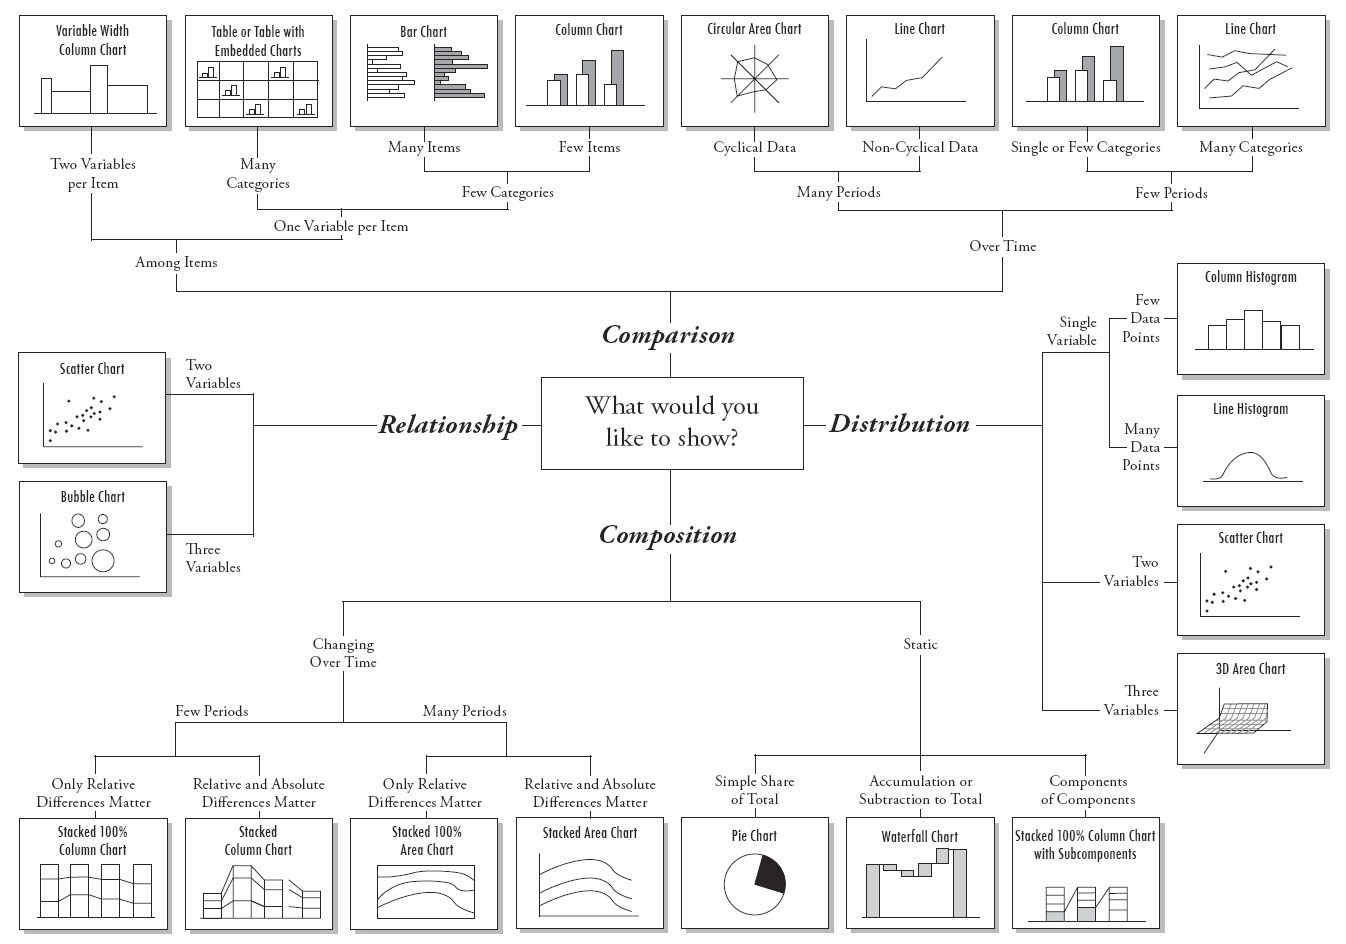
\includegraphics[width=\textwidth]{image3.png}
    \caption{Tipos de gráficos e a sua adequação a diferentes objetivos de análise \citep{abela2006}.}
    \label{fig:tipos_graficos}
\end{figure}

% ---- 4.2 Teste B ----
\section{Teste B}
\label{sec:teste_b}

% Repetir a estrutura anterior para cada teste realizado.
Descrever o objetivo, a preparação, a execução e os resultados do teste B.

% ---- 4.x Teste \ldots ----
% \section{Teste \ldots}
% \label{sec:teste_x}
% Repetir para cada teste adicional.

% ---- Discussão 

% Cap. 5 — Conclusões
% =============================================================================
% Template LaTeX IPG  —  https://github.com/VagnerBomJesus/TEMPLATE-IPG-LATEX
% Autor base, criador e mantenedor do projeto:
%     Vagner Bom Jesus  (@VagnerBomJesus)
%
% Proprietario e autor original deste template. Ao reutilizar, distribuir ou
% editar, MANTER este credito ao autor base (nao remover). Quem usa o template
% e o autor do SEU relatorio; o criador base do modelo e Vagner Bom Jesus.
% Licenca: GPL-3.0 (ver LICENSE).
% =============================================================================

% =============================================================================
% Capítulo 5 — Conclusões
% =============================================================================

\chapter{Conclusões}
\label{cap:conclusoes}

% Responder às seguintes questões:
% - Qual é o resumo do projeto (problema e solução)?
% - Qual é o resumo dos testes e resultados?
% - Quais são as limitações do trabalho?
% - O que ficou por fazer?
Este capítulo apresenta as conclusões do trabalho, as principais contribuições, as limitações identificadas e sugestões de trabalho futuro.

% ---- 5.1 Síntese do Trabalho ----
\section{Síntese do Trabalho}
\label{sec:sintese}

% Resumir o projeto: o problema abordado, a solução implementada e os
% principais resultados dos testes.
Apresentar uma síntese do trabalho realizado, recordando os objetivos propostos e os resultados alcançados.

% ---- 5.2 Contribuições ----
\section{Contribuições}
\label{sec:contribuicoes}

Identificar as principais contribuições do trabalho.

\begin{itemize}
    \item Contribuição 1
    \item Contribuição 2
    \item Contribuição 3
\end{itemize}

% ---- 5.3 Limitações ----
\section{Limitações}
\label{sec:limitacoes}

% Descrever o que o sistema não faz ou faz de forma limitada,
% e que pode ser melhorado no futuro.
Identificar as limitações do trabalho.

% ---- 5.4 Trabalho Futuro ----
\section{Trabalho Futuro}
\label{sec:trabalho_futuro}

% Descrever o que ficou por fazer, melhorias possíveis e
% direções de investigação futura.
Sugerir possíveis direções para trabalho futuro.

\begin{itemize}
    \item Melhoria 1
    \item Funcionalidade adicional 1
    \item Investigação futura 1
\end{itemize}


% ---- BACKMATTER ----
\backmatter

% Referências bibliográficas
% =============================================================================
% Template LaTeX IPG  —  https://github.com/VagnerBomJesus/TEMPLATE-IPG-LATEX
% Autor base, criador e mantenedor do projeto:
%     Vagner Bom Jesus  (@VagnerBomJesus)
%
% Proprietario e autor original deste template. Ao reutilizar, distribuir ou
% editar, MANTER este credito ao autor base (nao remover). Quem usa o template
% e o autor do SEU relatorio; o criador base do modelo e Vagner Bom Jesus.
% Licenca: GPL-3.0 (ver LICENSE).
% =============================================================================

% =============================================================================
% Referências Bibliográficas — NP 405 / Autor-Data
%
% Regras:
% - Ordenadas alfabeticamente pelo último nome do primeiro autor
% - Evitar referências sem revisão científica adequada
% - Situações de uso obrigatório:
%     1. Referência a trabalhos de outros autores
%     2. Opiniões/conclusões/dados/figuras/tabelas de outros
%     3. Informação técnica suplementar (fichas técnicas, manuais de API, etc.)
% - Espera-se algumas dezenas de referências num relatório de mestrado
% =============================================================================

\cleardoublepage
\phantomsection
\addcontentsline{toc}{chapter}{Referências Bibliográficas}

% \nocite{*} imprime TODAS as entradas do referencias.bib,

% Anexos
% =============================================================================
% Template LaTeX IPG  —  https://github.com/VagnerBomJesus/TEMPLATE-IPG-LATEX
% Autor base, criador e mantenedor do projeto:
%     Vagner Bom Jesus  (@VagnerBomJesus)
%
% Proprietario e autor original deste template. Ao reutilizar, distribuir ou
% editar, MANTER este credito ao autor base (nao remover). Quem usa o template
% e o autor do SEU relatorio; o criador base do modelo e Vagner Bom Jesus.
% Licenca: GPL-3.0 (ver LICENSE).
% =============================================================================

% =============================================================================
% Anexos
% Adicionar como anexos documentos produzidos ou não pelo autor que incluam
% informação complementar referenciada no relatório.
% =============================================================================

\cleardoublepage
\appendix
\addcontentsline{toc}{chapter}{Anexos}

\chapter{Anexo A}
\label{anx:a}

% Descrever o conteúdo do Anexo A (ex.: questionários, formulários,
% diagramas adicionais, código fonte complementar, etc.)
Incluir aqui material suplementar relevante para o trabalho.

% Para incluir um PDF como anexo:
% \includepdf[pages=-]{ficheiro.pdf}

\chapter{Anexo B}
\label{anx:b}

% Descrever o conteúdo do Anexo B.
Incluir aqui o conteúdo do segundo anexo.

% \chapter{Anexo C}
% \label{anx:c}
% Adicionar mais anexos conforme necessário.


\end{document}
